\chapter{Topological HLT Development at $\sqrt{s}=13 \TeV$}
\label{ch:hlt13TeV}

To target a broad range of new physics possibilities, we designed four different
types of triggers for use at $\sqrt{s}=13\TeV$:
\begin{itemize}
\item Dijet razor trigger with hyperbolic \MR and \Rtwo requirements targetting the squark pair production topology;
\item Quadjet razor trigger with hyperbolic \MR and \Rtwo requirements
  targetting top-squark or gluino pair production topologies;
\item High-\Rtwo trigger targetting dijet+invisible topologies with
  large transverse momentum imbalance; and
\item Razor $\PH(\PQb\bar\PQb)$ trigger targetting production of
  $\PH+\mathrm{jet}+\mathrm{invisible}$ with some transverse momentum imbalance.
\end{itemize}

The dijet and quadjet razor triggers are broadly motivated by SUSY pair
production and represent an update and improvement of the razor triggers
used in previous searches at $\sqrt{s}=8\TeV$~\cite{razor8TeV}. Both
sets of triggers are based on hyperbolic thresholds in the $(\MR,\Rtwo)$
plane, with the 2015 updated thresholds shown in
Fig~\ref{fig:hyperbolic}. The 2015 hyperbolic contours follow the
iso-probability contours derived from the background-only fit to the MultiJet category
in the 8\TeV razor search performed using 2012 data. This implies
these hyperbolic contours efficiently reject background, while
maintaining a large signal acceptance. 

\begin{figure}[ht!]
\centering
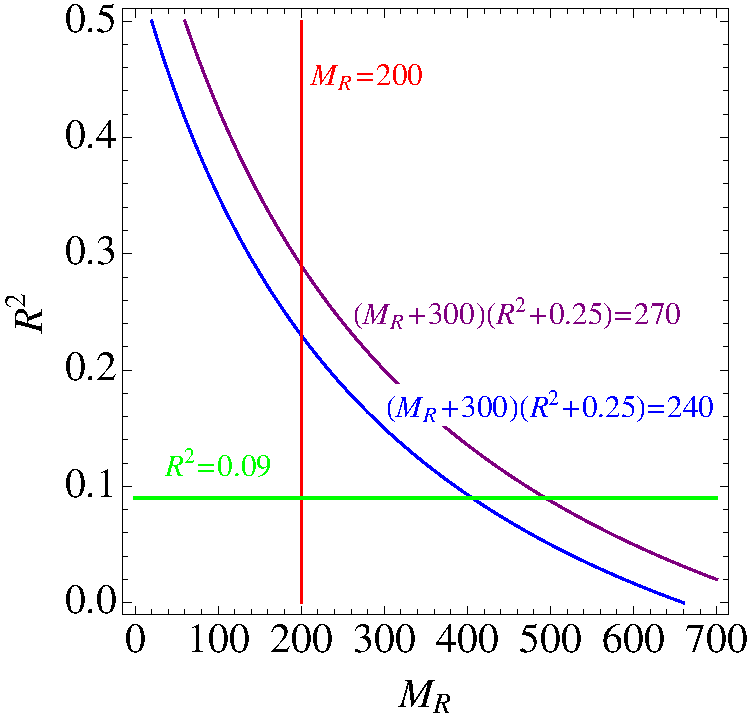
\includegraphics[width=0.49\textwidth]{figs/hlt13TeV/HLTRsqMR.pdf}
\caption{\label{fig:hyperbolic} Hyperbolic and baseline thresholds in
  \Rtwo and \MR used in the dijet and quadjet razor triggers.}
\end{figure}

Another update is that the 13 \TeV razor triggers are based on PF-reconstructed objects rather
than Calo jets and muons, which means the online $\Rtwo$ variable is
much more correlated with the offline $\Rtwo$ variable, which is also
PF-based. This leads to an improved trigger efficiency for 2015, shown in Fig.~\ref{fig:turnons}

\begin{figure}[ht!]
\centering
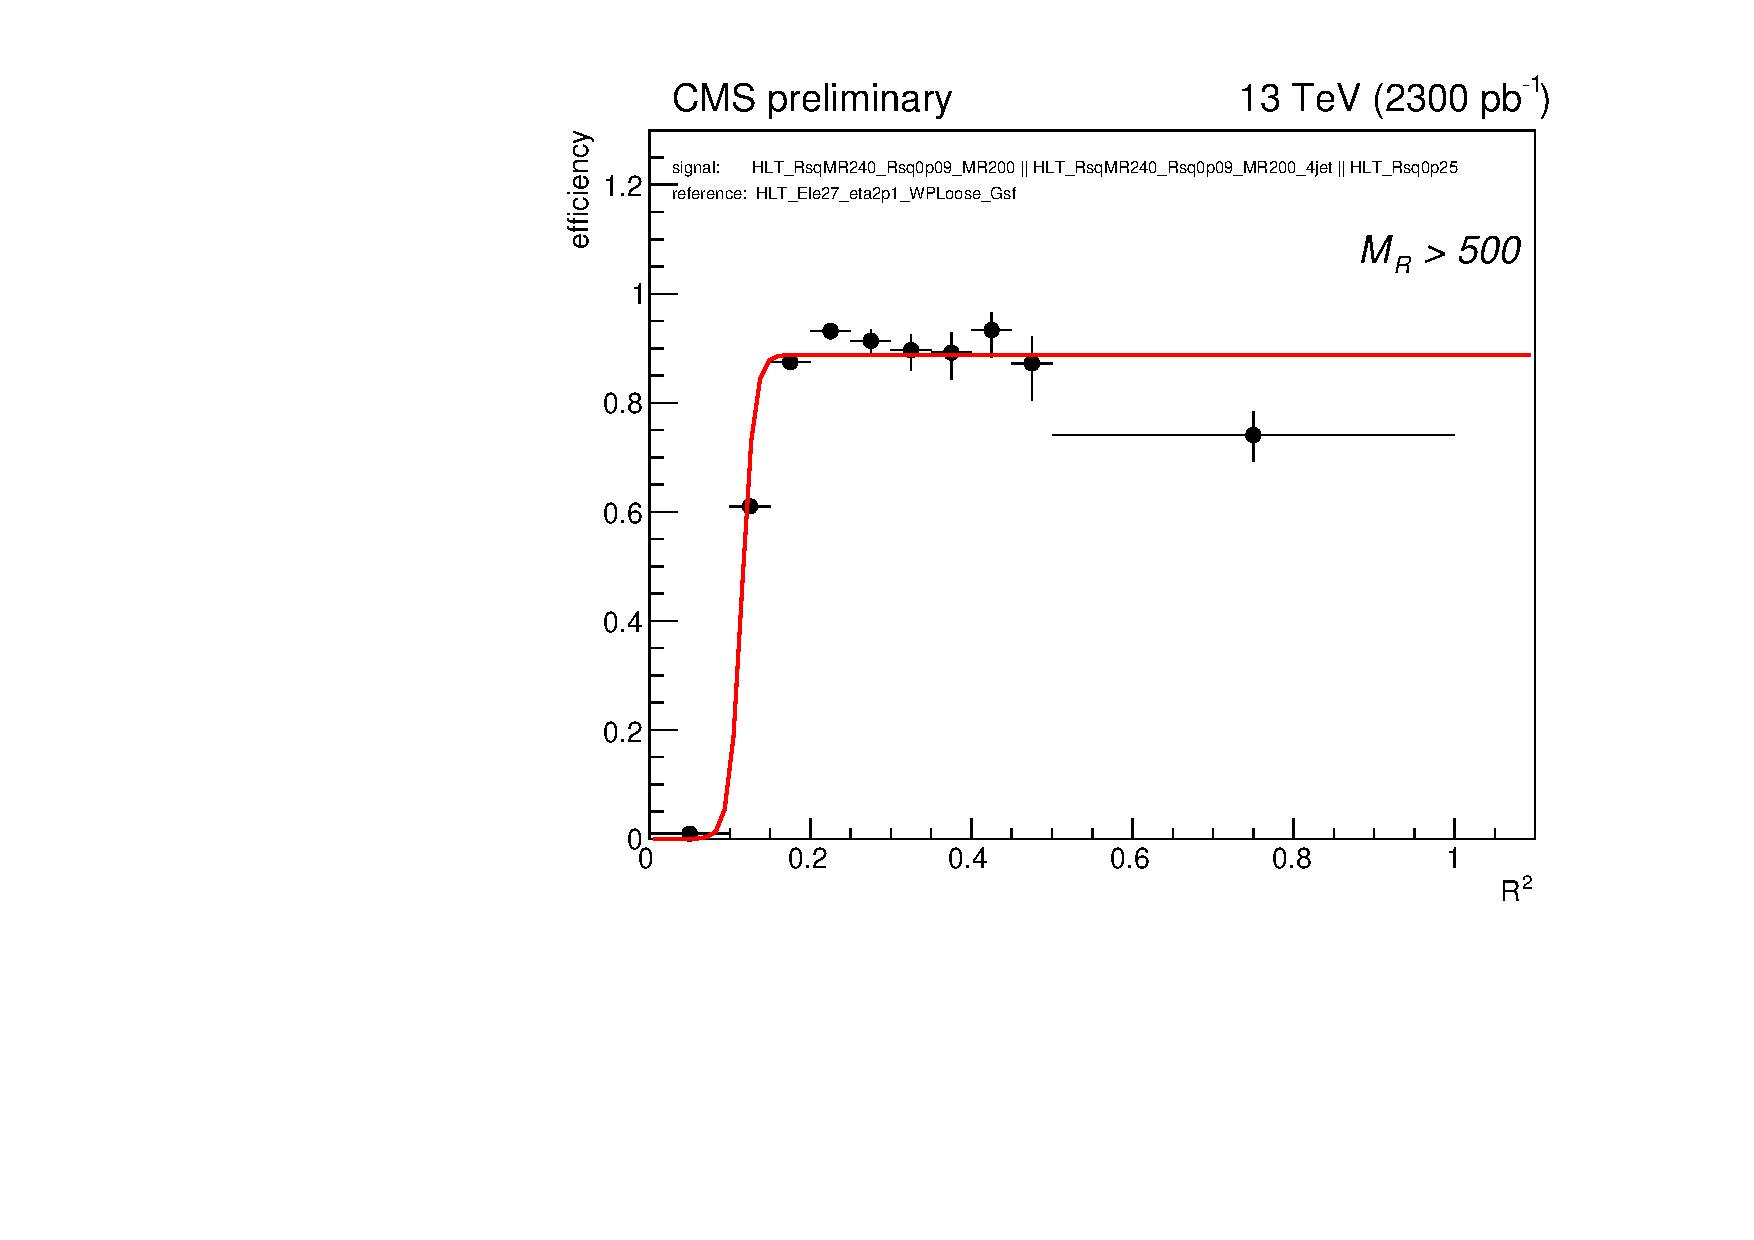
\includegraphics[width=0.45\textwidth]{figs/hlt13TeV/turnons_2015_no100GeVmuons/HLT_RsqMR240_Rsq0p09_MR200_HLT_RsqMR240_Rsq0p09_MR200_4jet_HLT_Rsq0p25_HLT_Ele27_eta2p1_WPLoose_Gsf_effRsq_MR500.pdf}
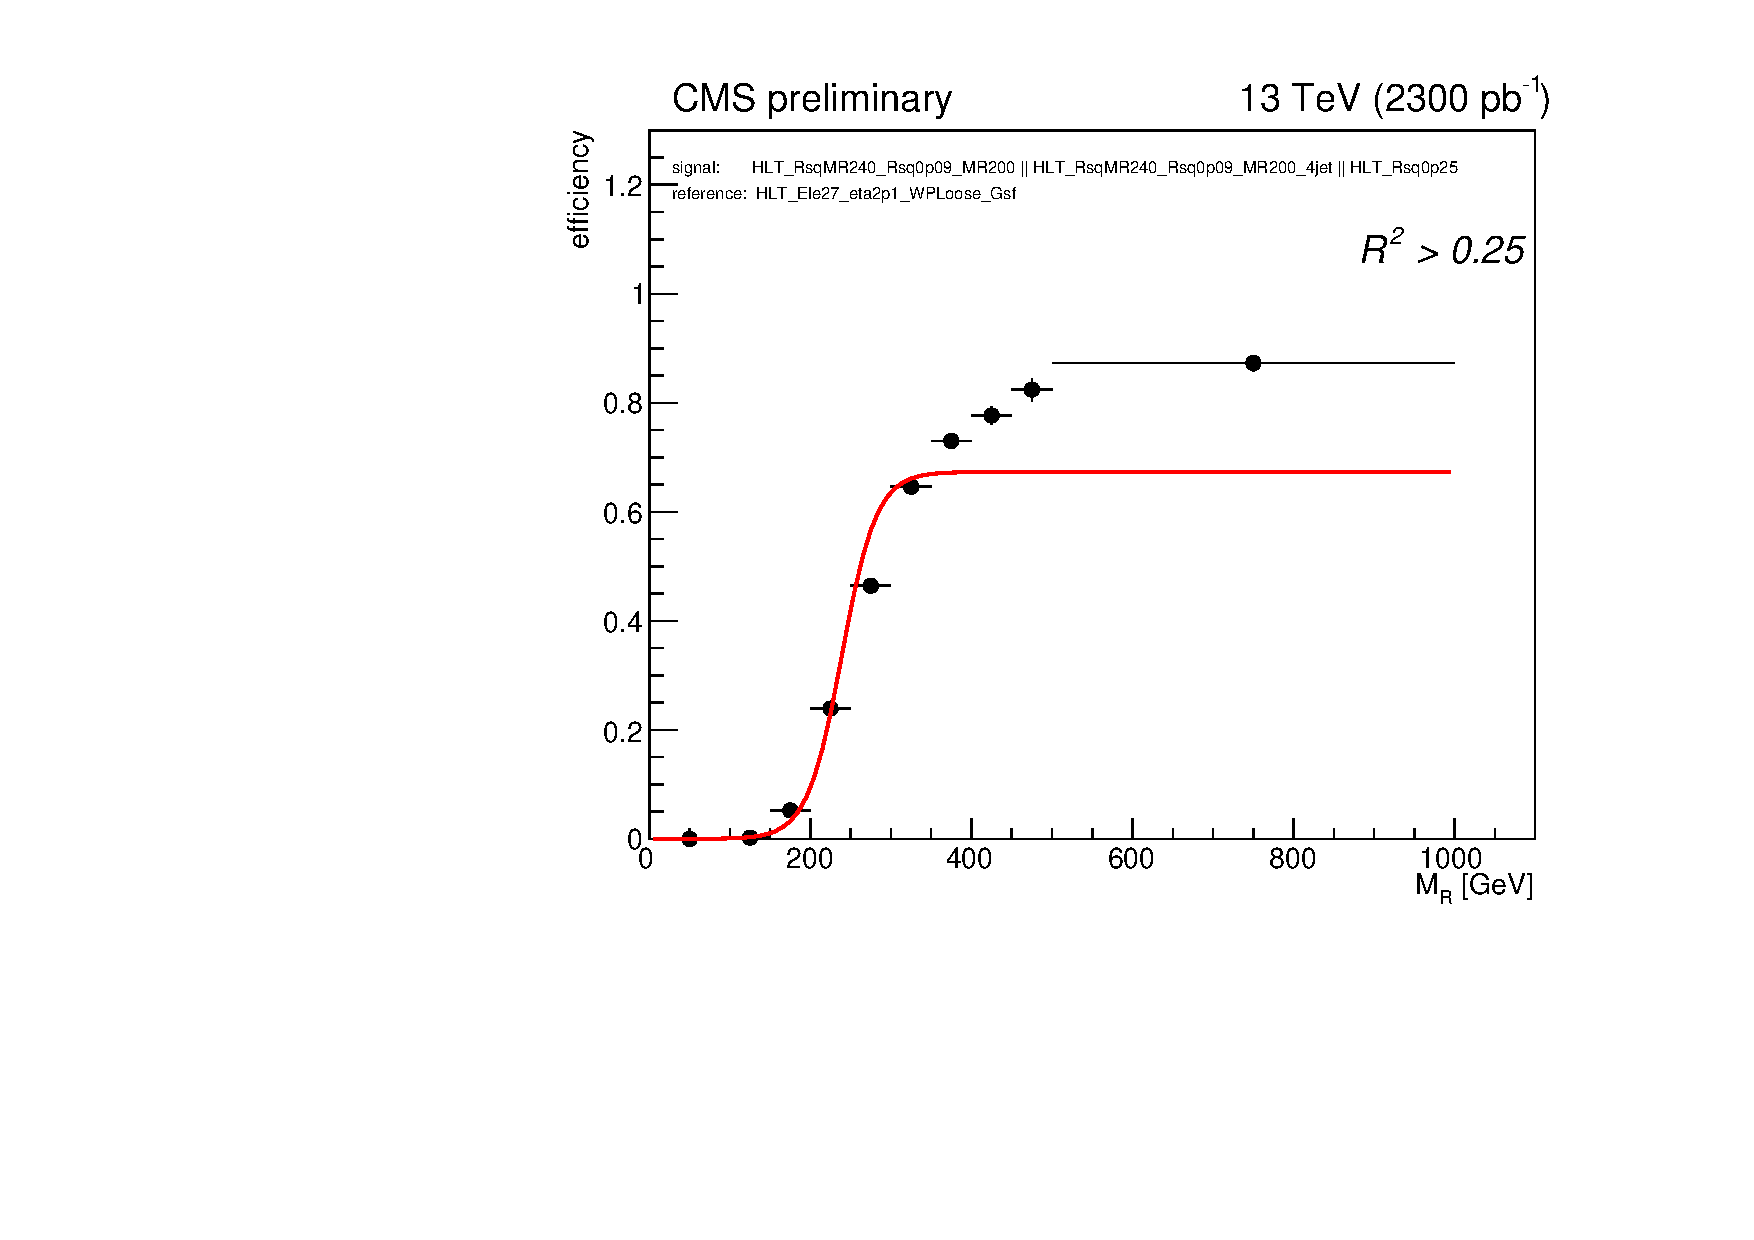
\includegraphics[width=0.45\textwidth]{figs/hlt13TeV/turnons_2015_no100GeVmuons/HLT_RsqMR240_Rsq0p09_MR200_HLT_RsqMR240_Rsq0p09_MR200_4jet_HLT_Rsq0p25_HLT_Ele27_eta2p1_WPLoose_Gsf_effMR_Rsq0p25.pdf}\\
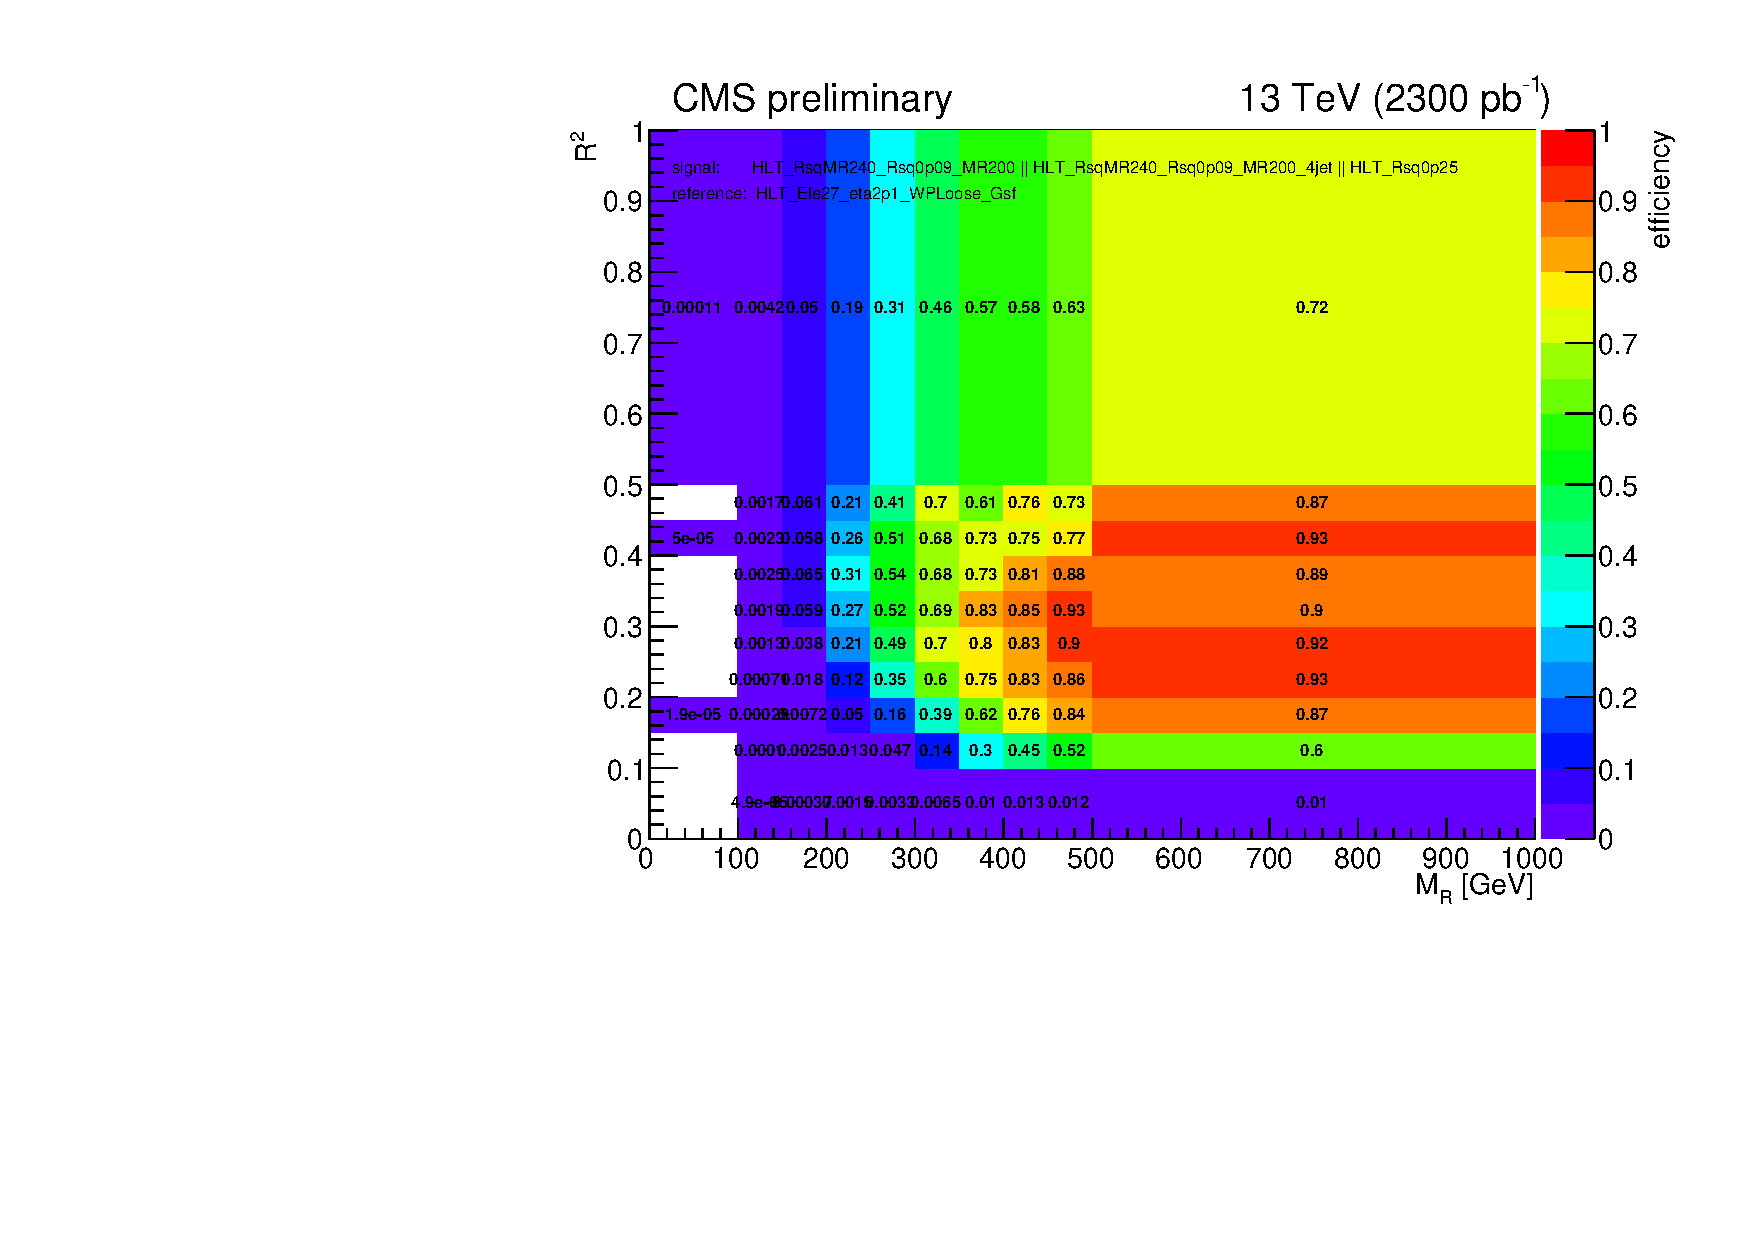
\includegraphics[width=0.45\textwidth]{figs/hlt13TeV/turnons_2015_no100GeVmuons/HLT_RsqMR240_Rsq0p09_MR200_HLT_RsqMR240_Rsq0p09_MR200_4jet_HLT_Rsq0p25_HLT_Ele27_eta2p1_WPLoose_Gsf_eff2D.pdf}
\caption{\label{fig:turnons} Trigger efficiencies for $\Rtwo$ (top
  left), $\MR$ (top right), and in the $(\MR,\Rtwo)$ plane (bottom).}
\end{figure}

\section{Design}


\begin{figure}[ht!]
\centering
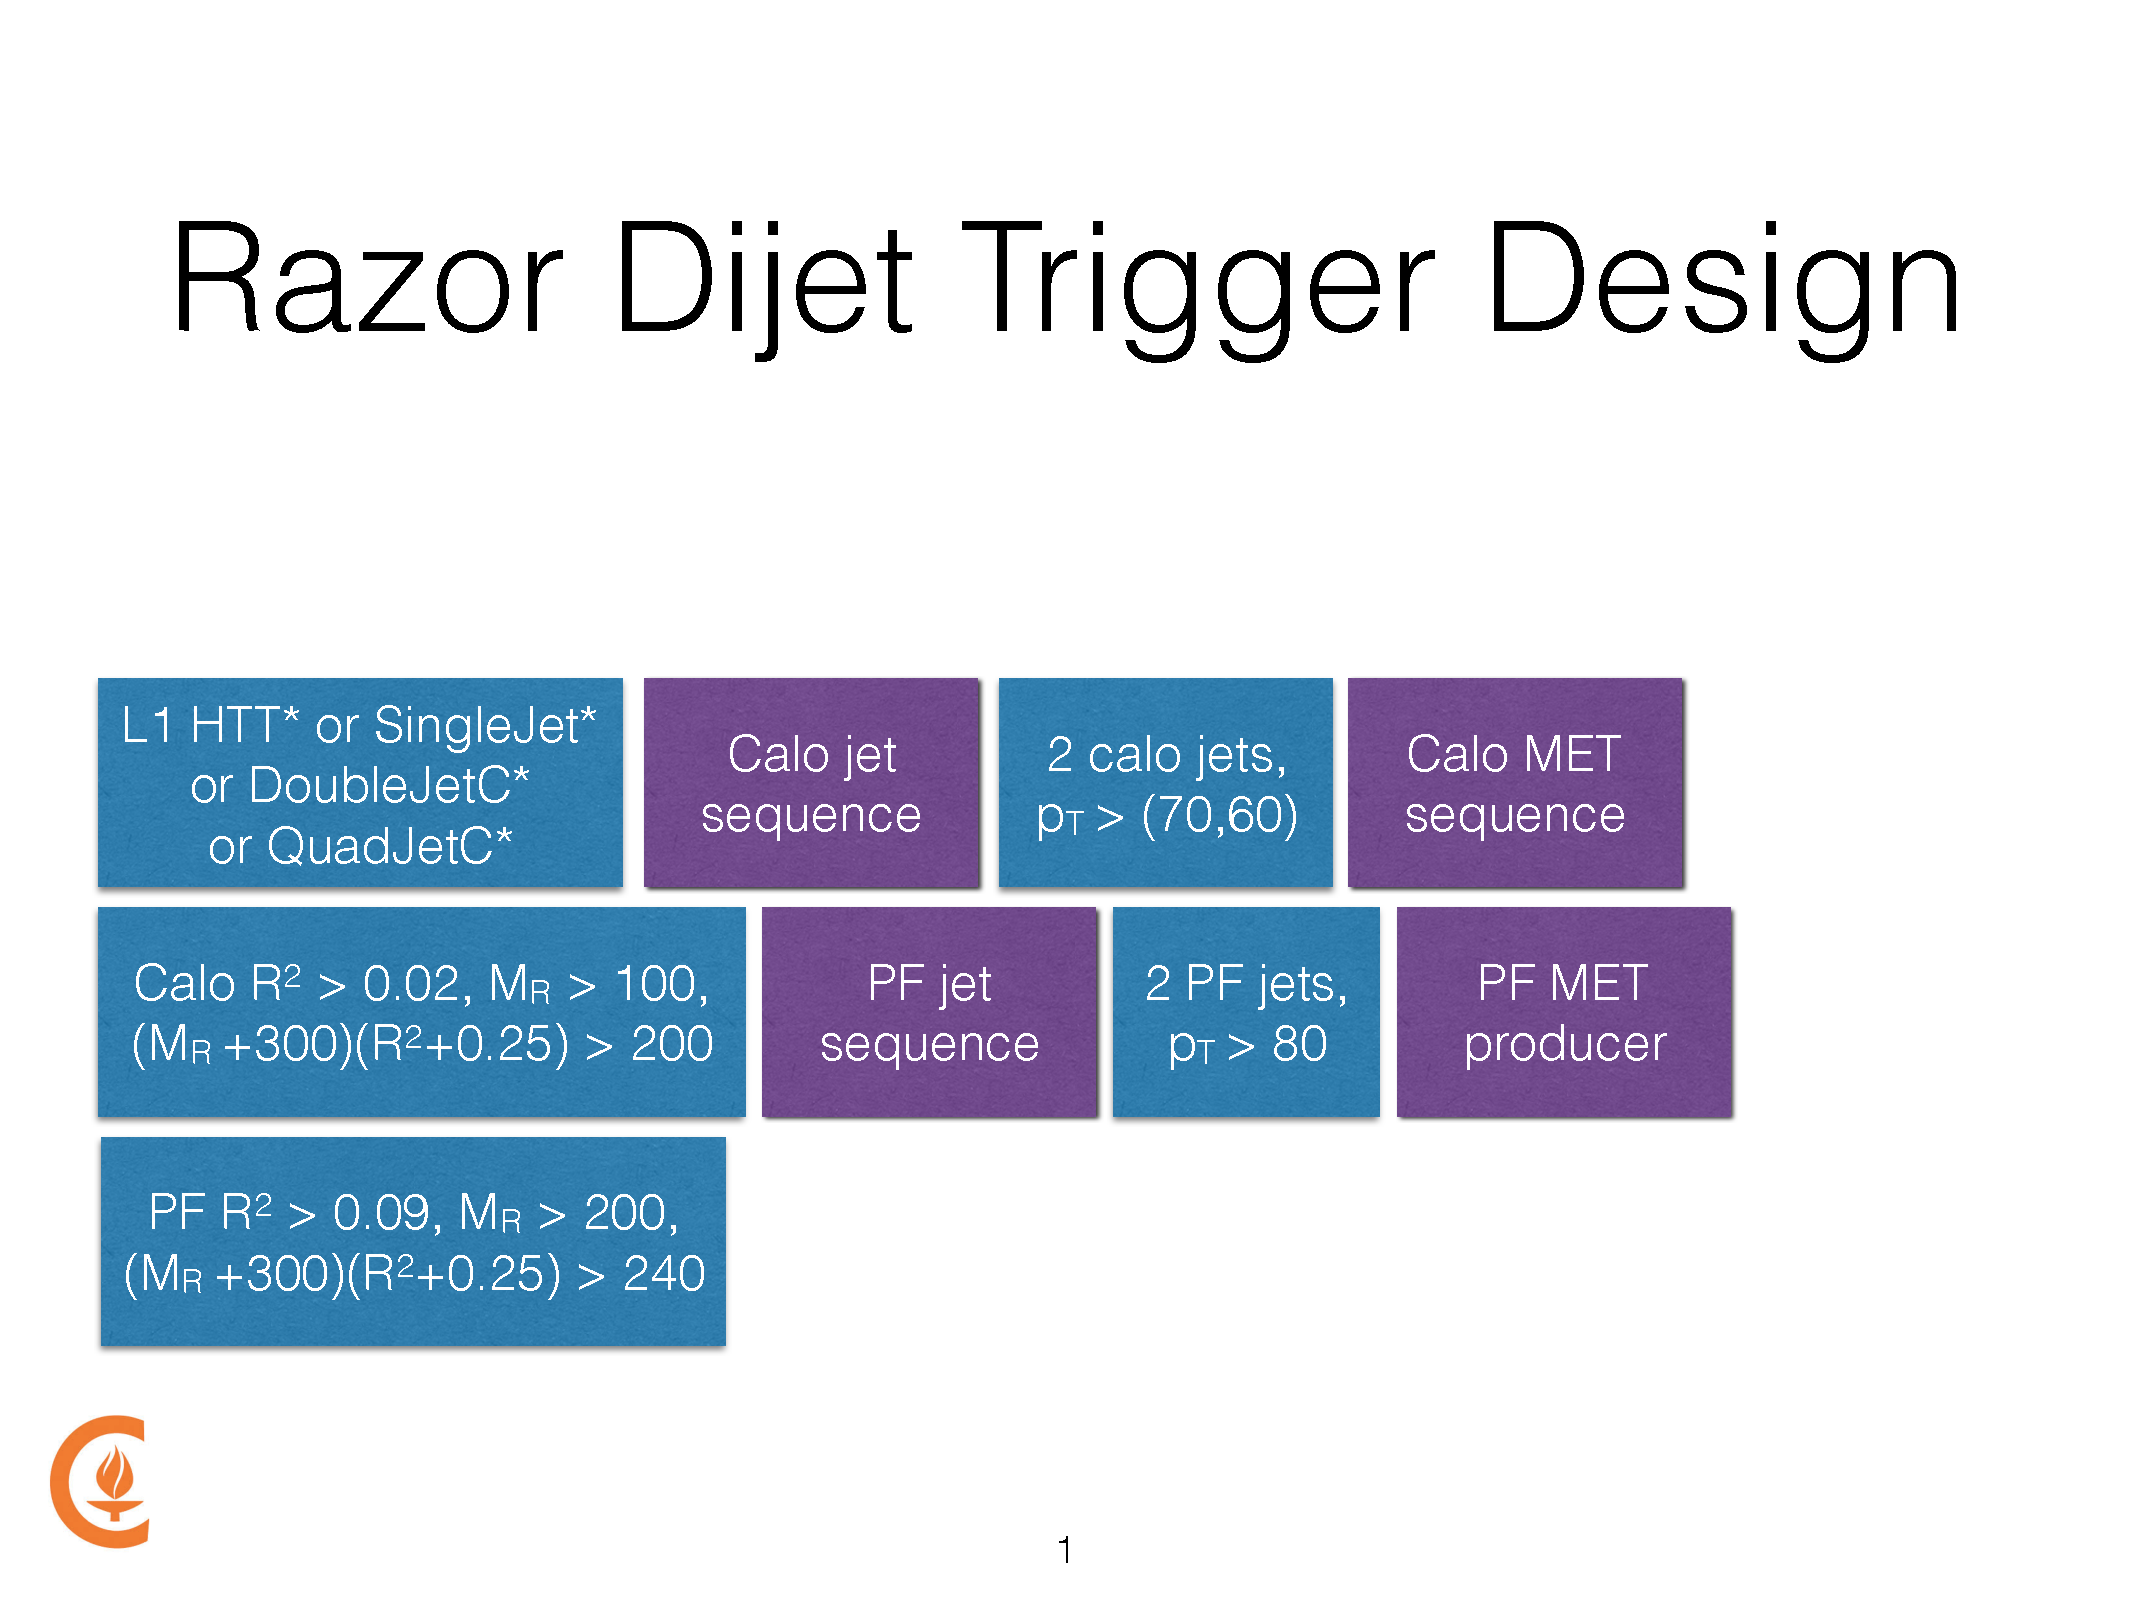
\includegraphics[width=0.8\textwidth,clip=true,viewport=0 110 1024
500]{figs/hlt13TeV/HLTDijetDesign.pdf}\\
(a)\\
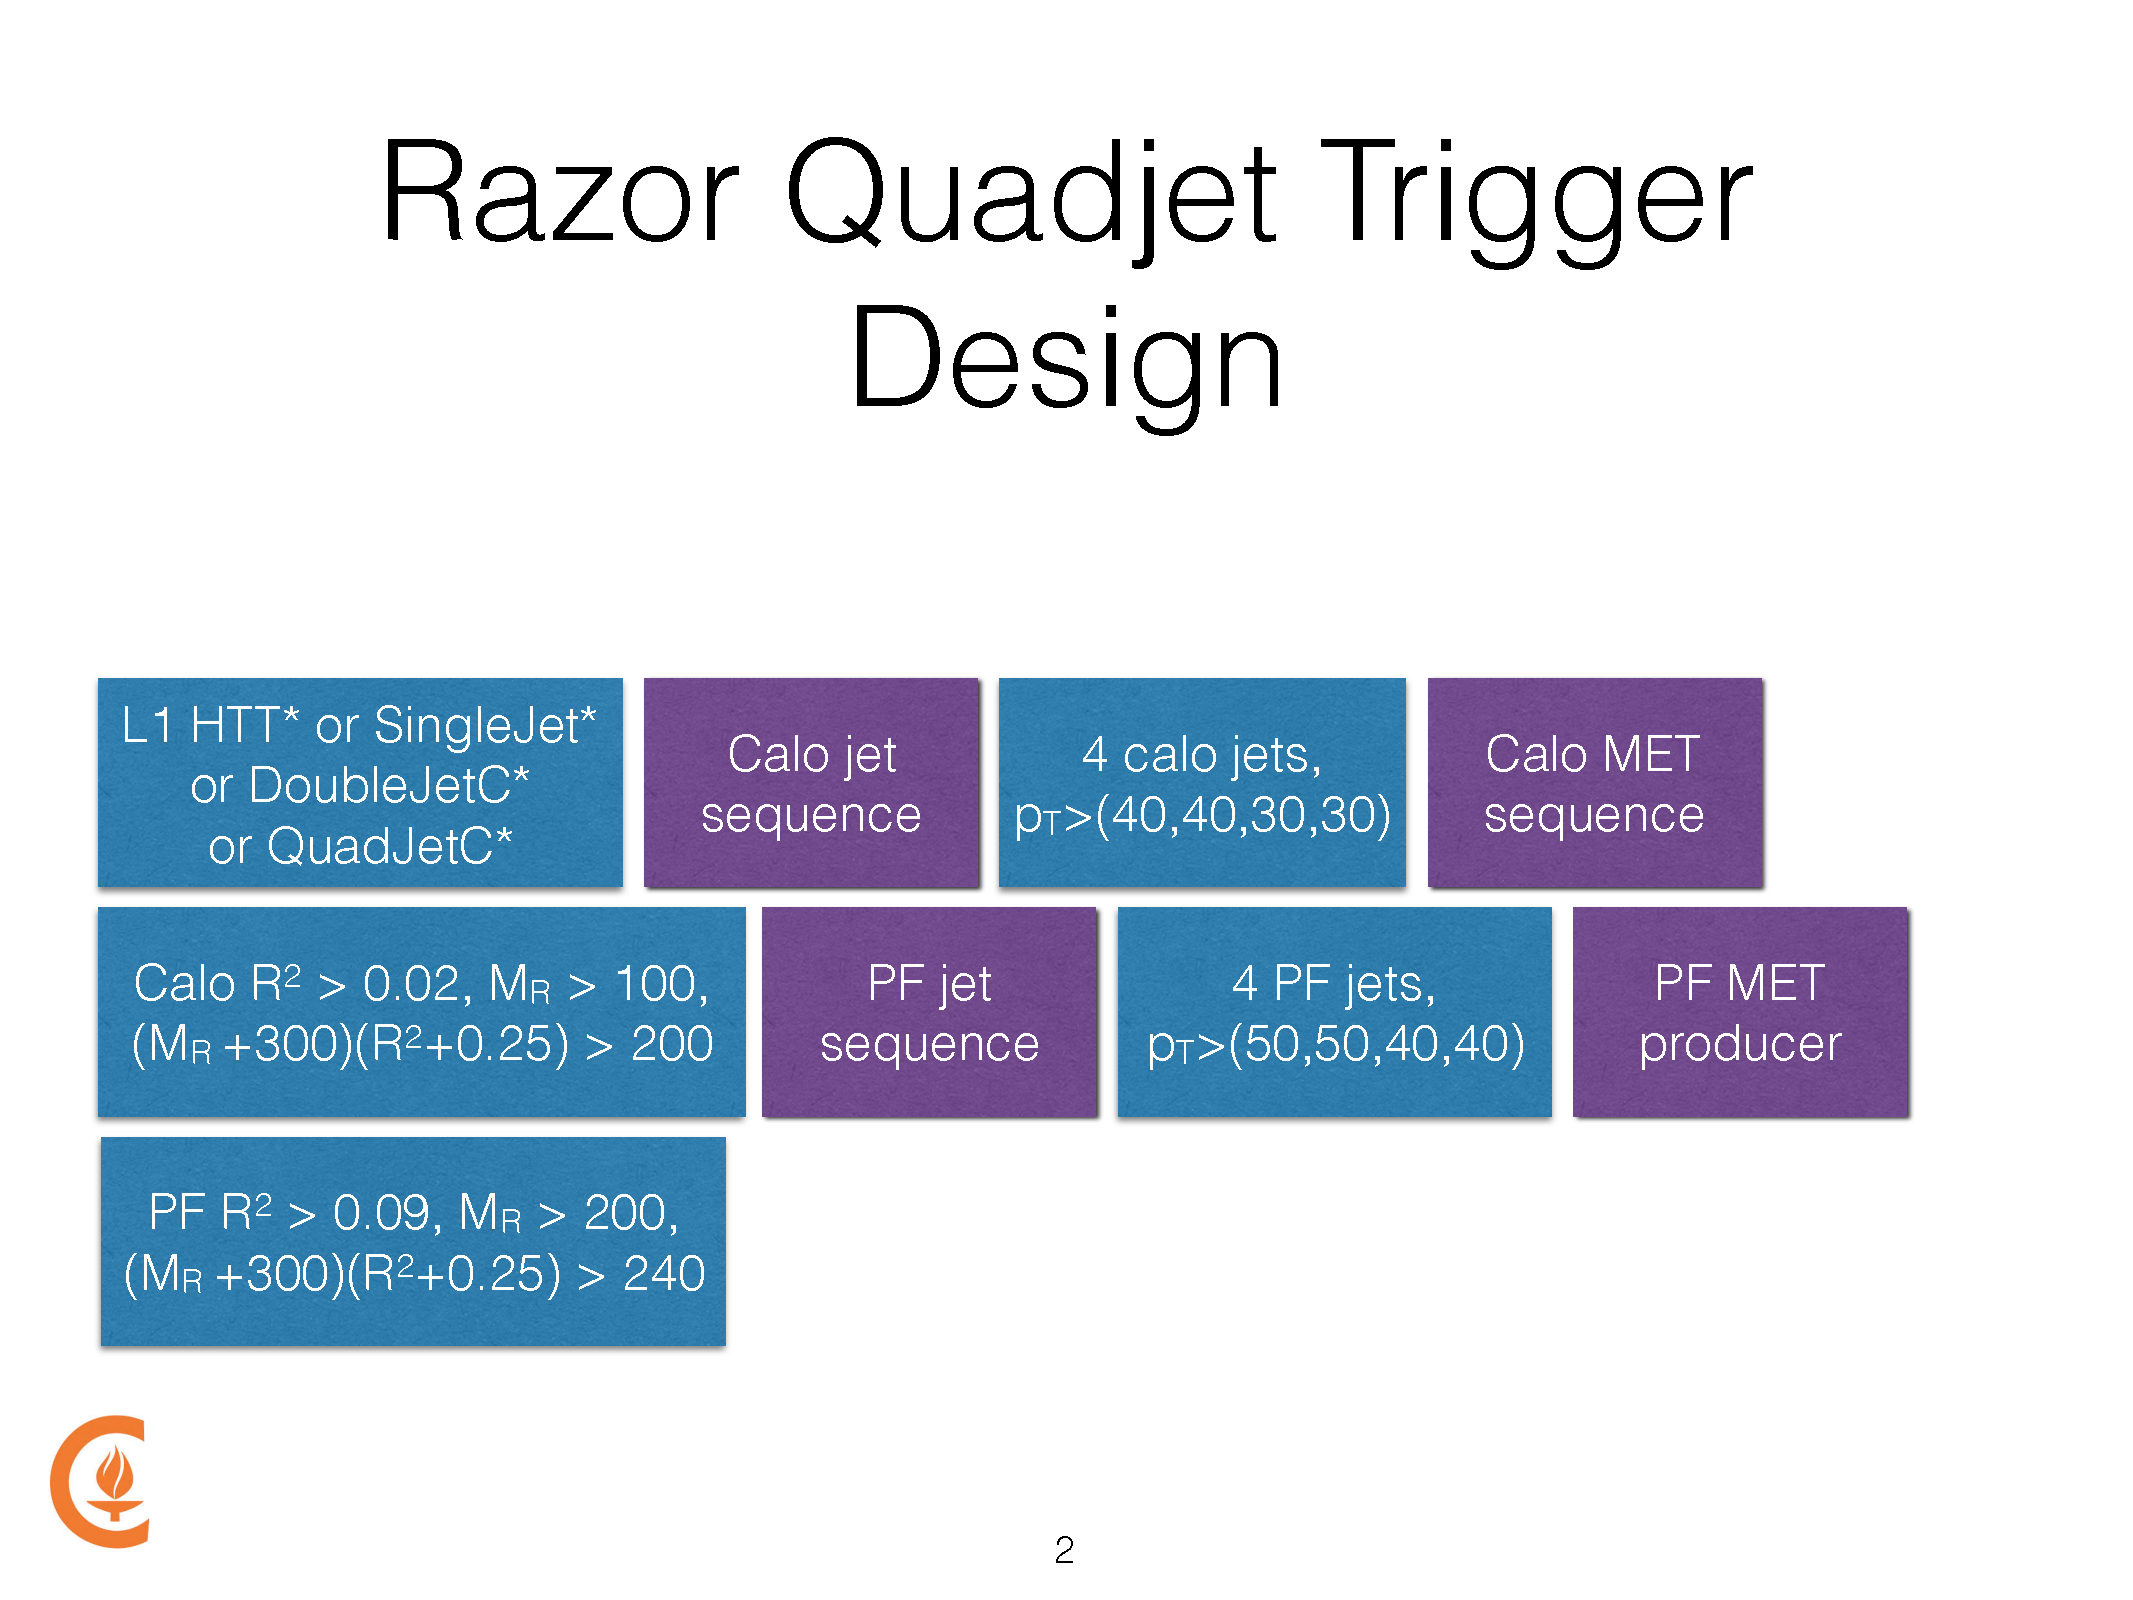
\includegraphics[width=0.8\textwidth,clip=true,viewport=0 110 1024
500]{figs/hlt13TeV/HLTQuadjetDesign.pdf}\\
(b)\\
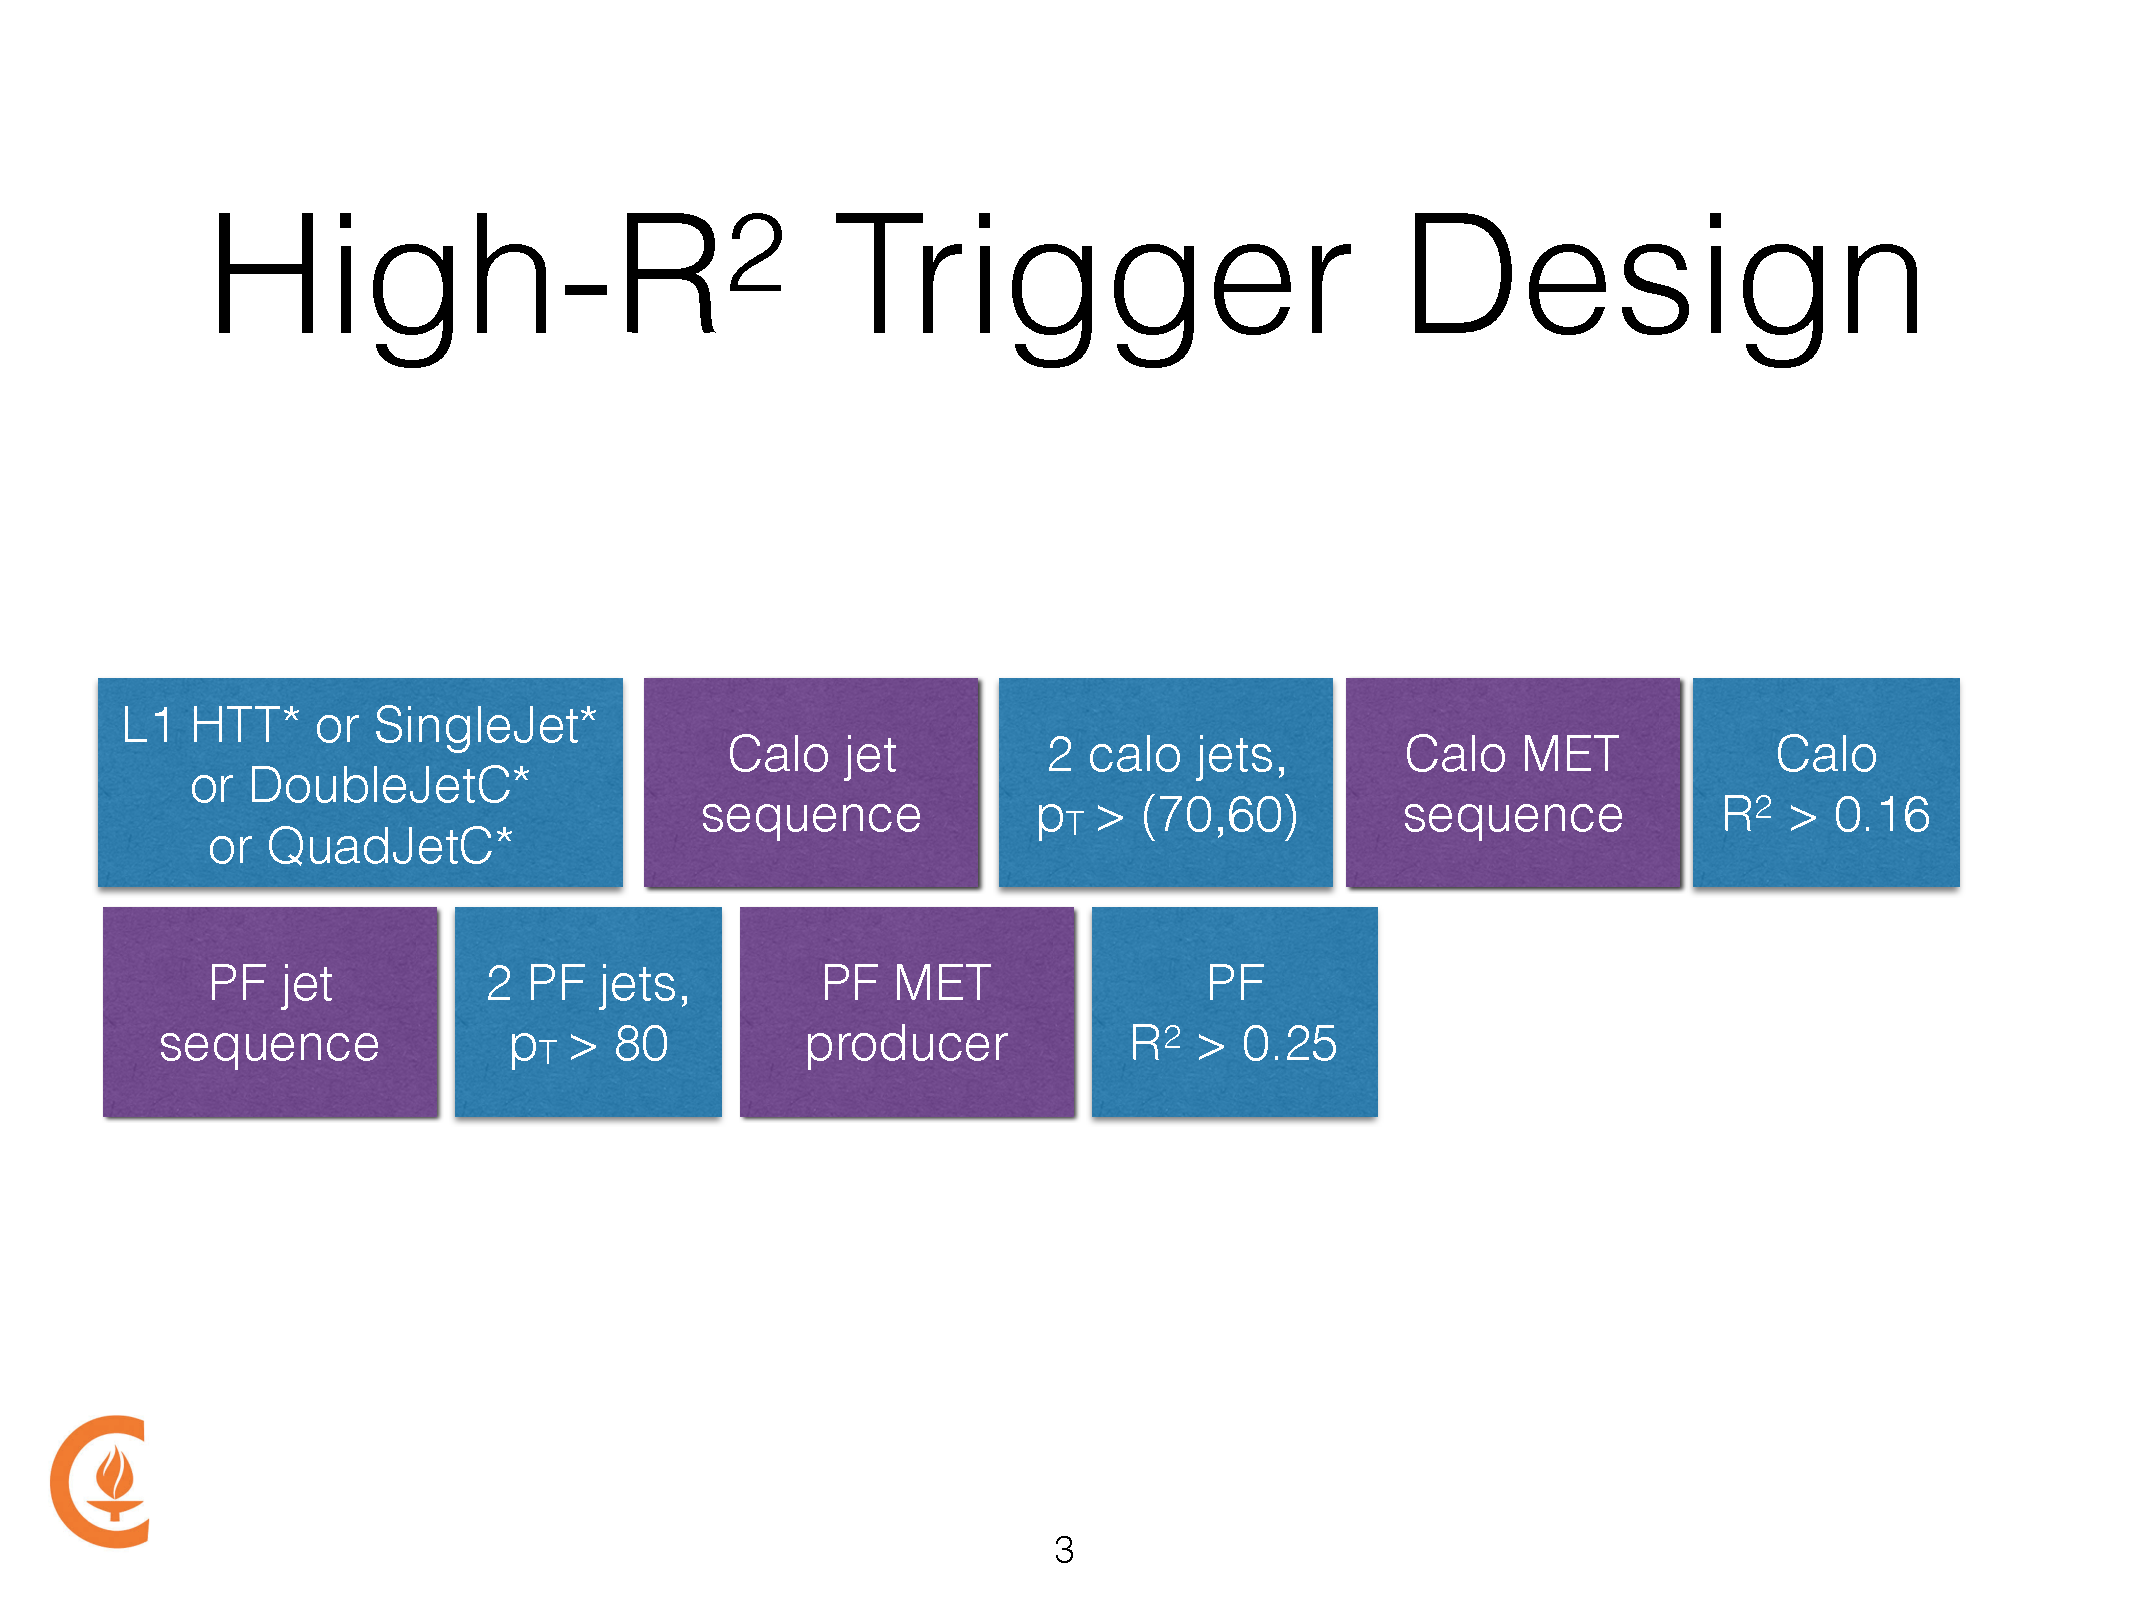
\includegraphics[width=0.8\textwidth,clip=true,viewport=0 220 1024
500]{figs/hlt13TeV/HLTR2Design.pdf}\\
(c)\\
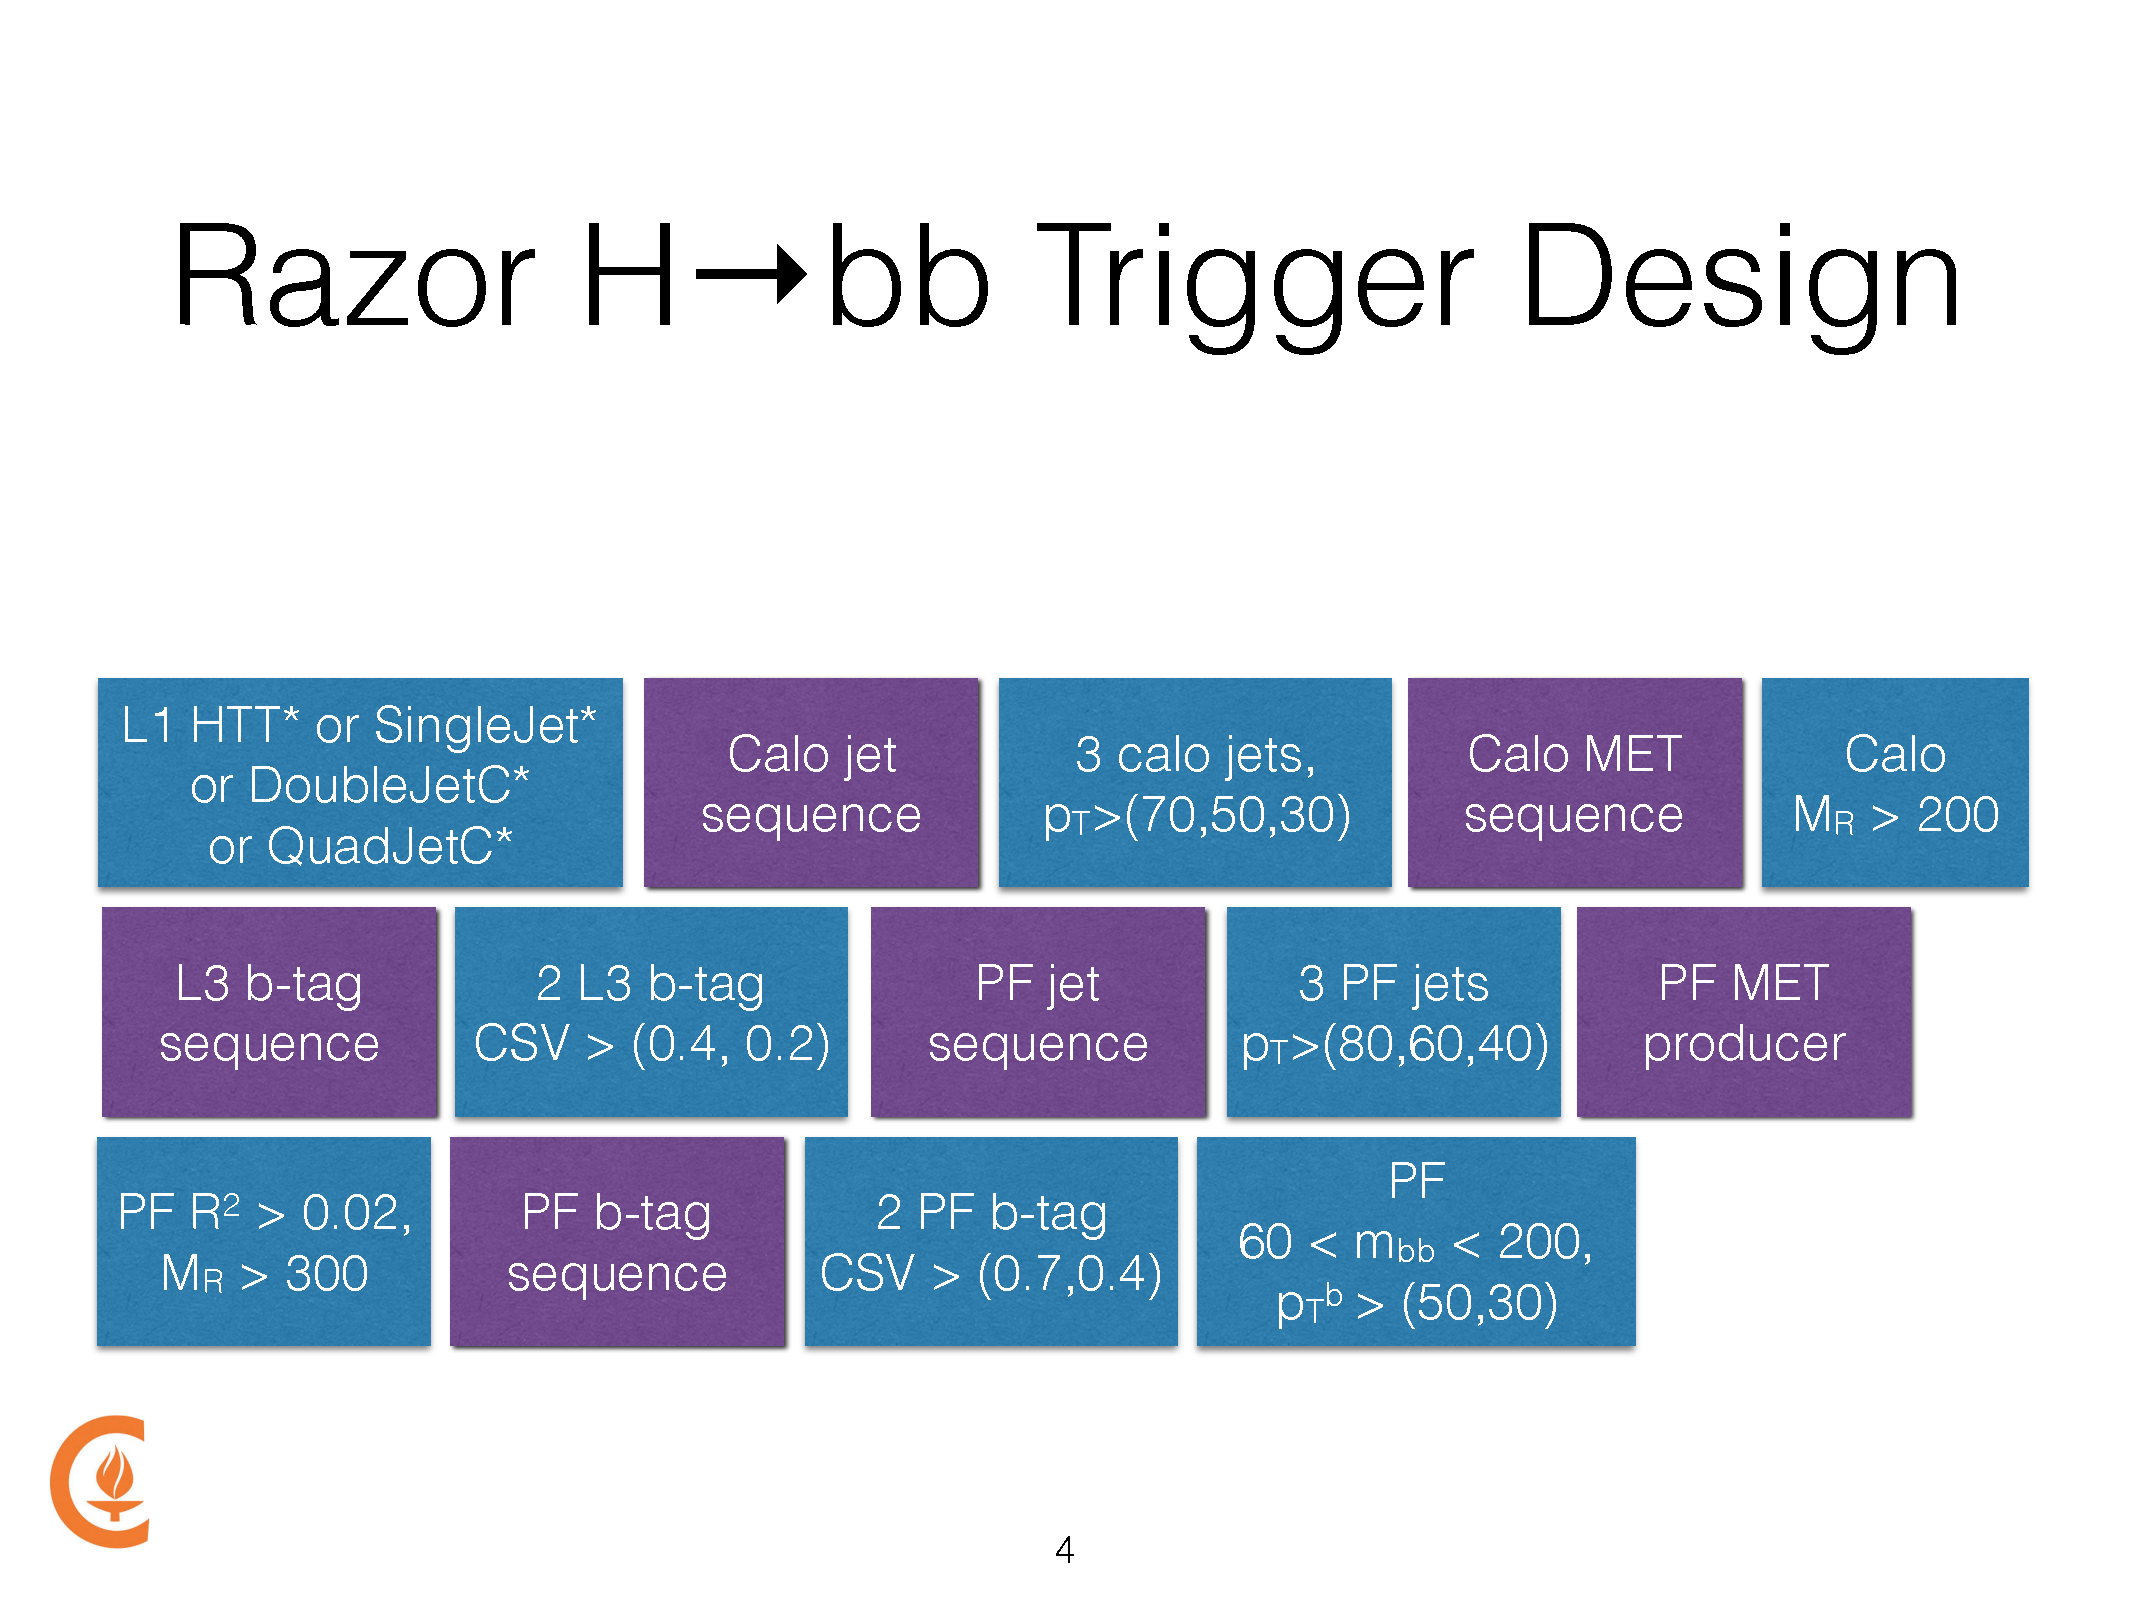
\includegraphics[width=0.8\textwidth,clip=true,viewport=0 110 1024
500]{figs/hlt13TeV/HLTRazorHbbDesign.pdf}\\
(d)
\caption{\label{fig:HLTdesign} Flow of the producer steps (in purple)
  and filter steps (in blue) in
  the razor triggers.}
\end{figure}

\section{HLT Rate and Timing estimates}

%\begin{table*}[ht!]
%\centering
% \caption{Rates for 0\unit{T} triggers.
% \label{tab:rates0T}}
%\resizebox{\textwidth}{!}{
%\begin{tabular}{l|l|l}
%\multirow{2}{*}{Trigger path} &  Data rate (run 260039) & MC rate (Spring '15) \\
% &  $4\times 10^{33}$ \unit{cm$^{-2}$ s$^{-1}$}, 17 PU &  \\\hline
%HLT\_Rsq0p25\_Calo & 3.7 Hz & \\
%HLT\_RsqMR240\_Rsq0p09\_MR200\_4jet\_Calo & 5.6 Hz & \\
%HLT\_RsqMR240\_Rsq0p09\_MR200\_Calo & 18.2 Hz & 
%\end{tabular}}
%\end{table*}

\begin{table*}[ht!]
\centering
 \caption{Rates for 2015 razor HLT paths at $5\times 10^{33}$ cm$^{-2}$
   s$^{-1}$ instantaneous luminosity with 17 average pileup events. \label{tab:rates2015}}
\resizebox{\textwidth}{!}{
\begin{tabular}{l|l|l}
\multirow{2}{*}{Trigger path} &  Data rate (run 260627) \\
 &  $5\times 10^{33}$ cm$^{-2}$ s$^{-1}$, 17 PU \\\hline
HLT\_Rsq0p02\_MR300\_TriPFJet80\_60\_40\_DoublePFBTagCSV0p7\_0p4\_Mbb60\_200& 16.0 Hz \\
HLT\_Rsq0p02\_MR300\_TriPFJet80\_60\_40\_DoublePFBTagCSV0p7\_Mbb60\_200 & 8.0 Hz \\
HLT\_Rsq0p25 & 0.7 Hz\\
HLT\_Rsq0p30 & 0.4 Hz \\
HLT\_RsqMR240\_Rsq0p09\_MR200\_4jet & 1.2 Hz \\
HLT\_RsqMR240\_Rsq0p09\_MR200 & 7.7 Hz \\
HLT\_RsqMR270\_Rsq0p09\_MR200\_4jet & 0.5 Hz \\
HLT\_RsqMR270\_Rsq0p09\_MR200 & 2.3 Hz 
\end{tabular}}
\end{table*}


\section{Pileup dependence}
Nominally, the trigger rate dependence on pileup is expected to be linear, but many
``sum'' quantities have a nonlinear dependence on pileup.

\begin{figure}[ht!]
\begin{tabular}{cc}
\centering 
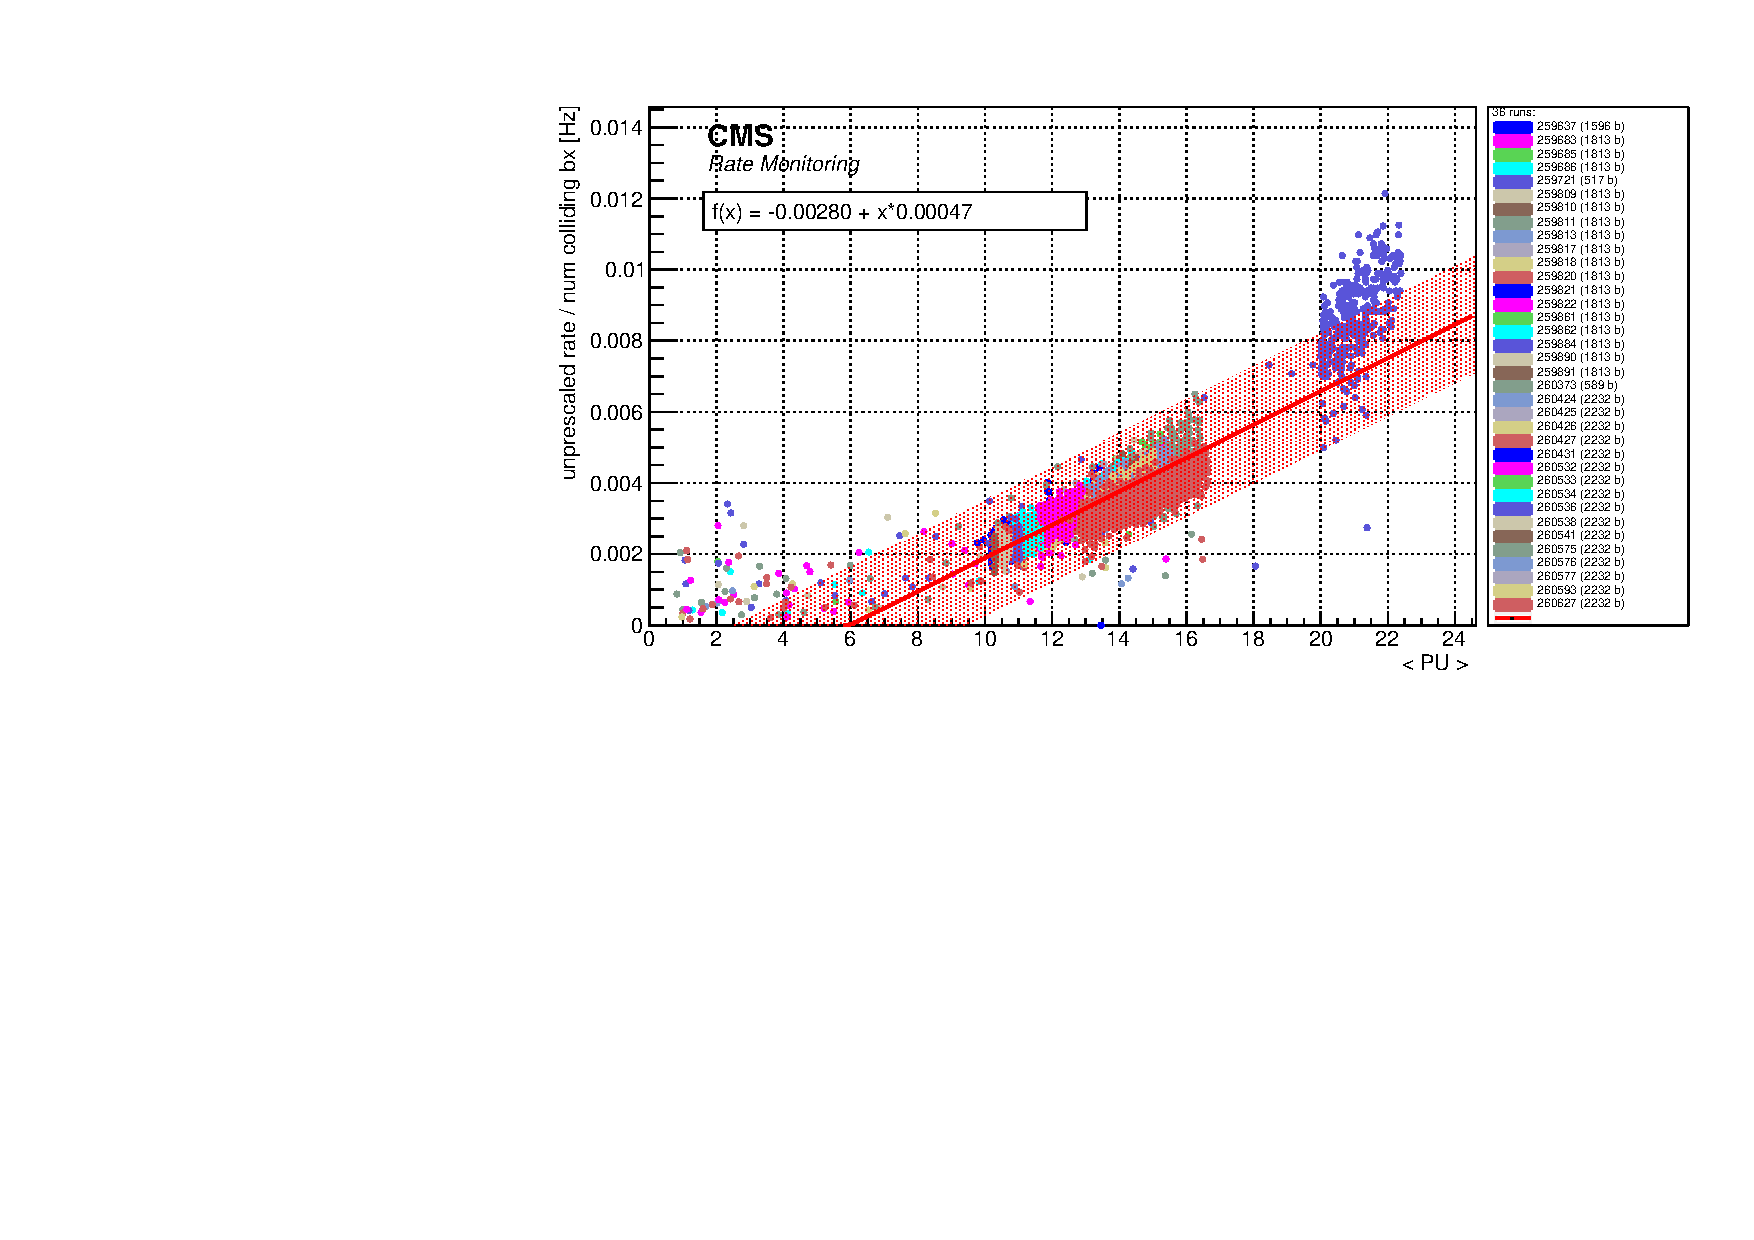
\includegraphics[width=0.49\textwidth]{figs/hlt13TeV/linear/HLT_RsqMR240_Rsq0p09_MR200_instLumi_vs_rawRate.pdf}
  & 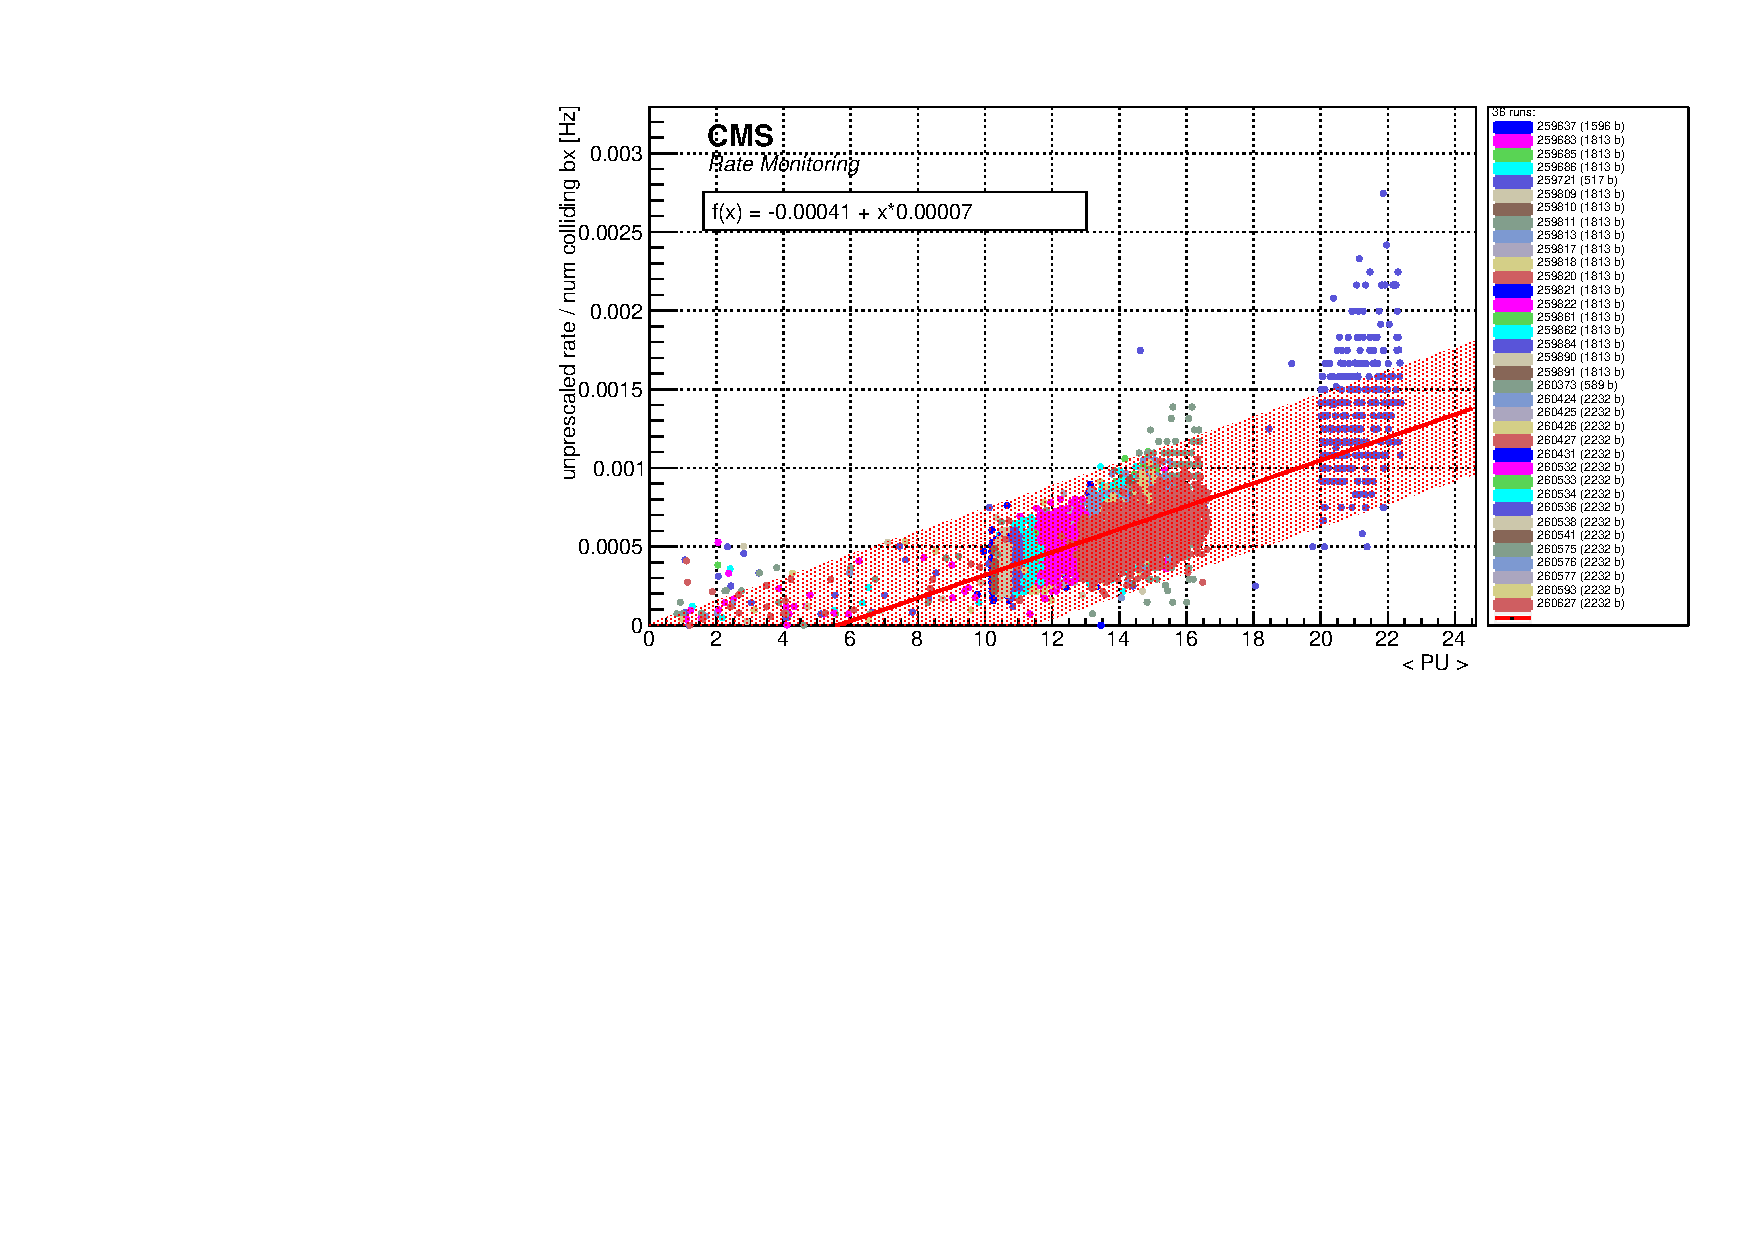
\includegraphics[width=0.49\textwidth]{figs/hlt13TeV/linear/HLT_RsqMR240_Rsq0p09_MR200_4jet_instLumi_vs_rawRate.pdf}\\
(a) & (b)\\
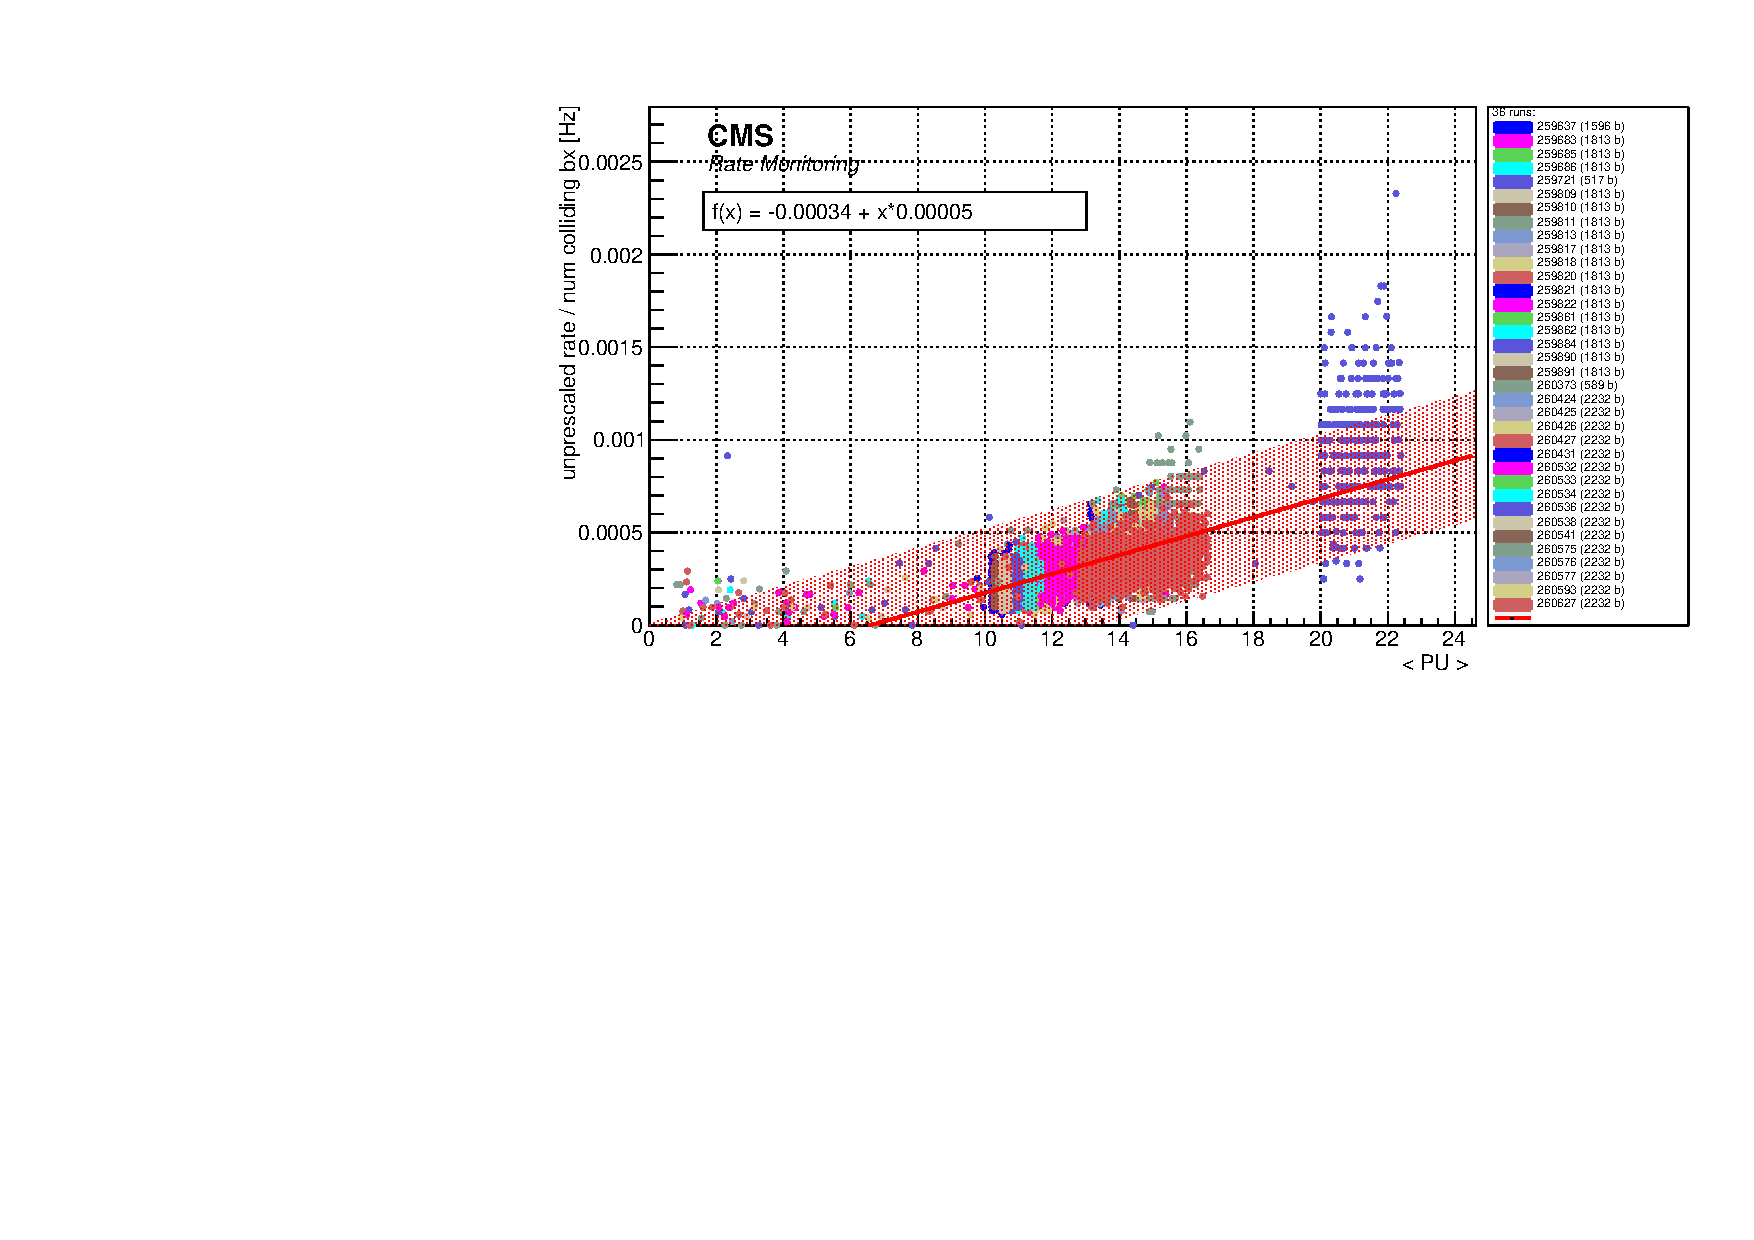
\includegraphics[width=0.49\textwidth]{figs/hlt13TeV/linear/HLT_Rsq0p25_instLumi_vs_rawRate.pdf}
  &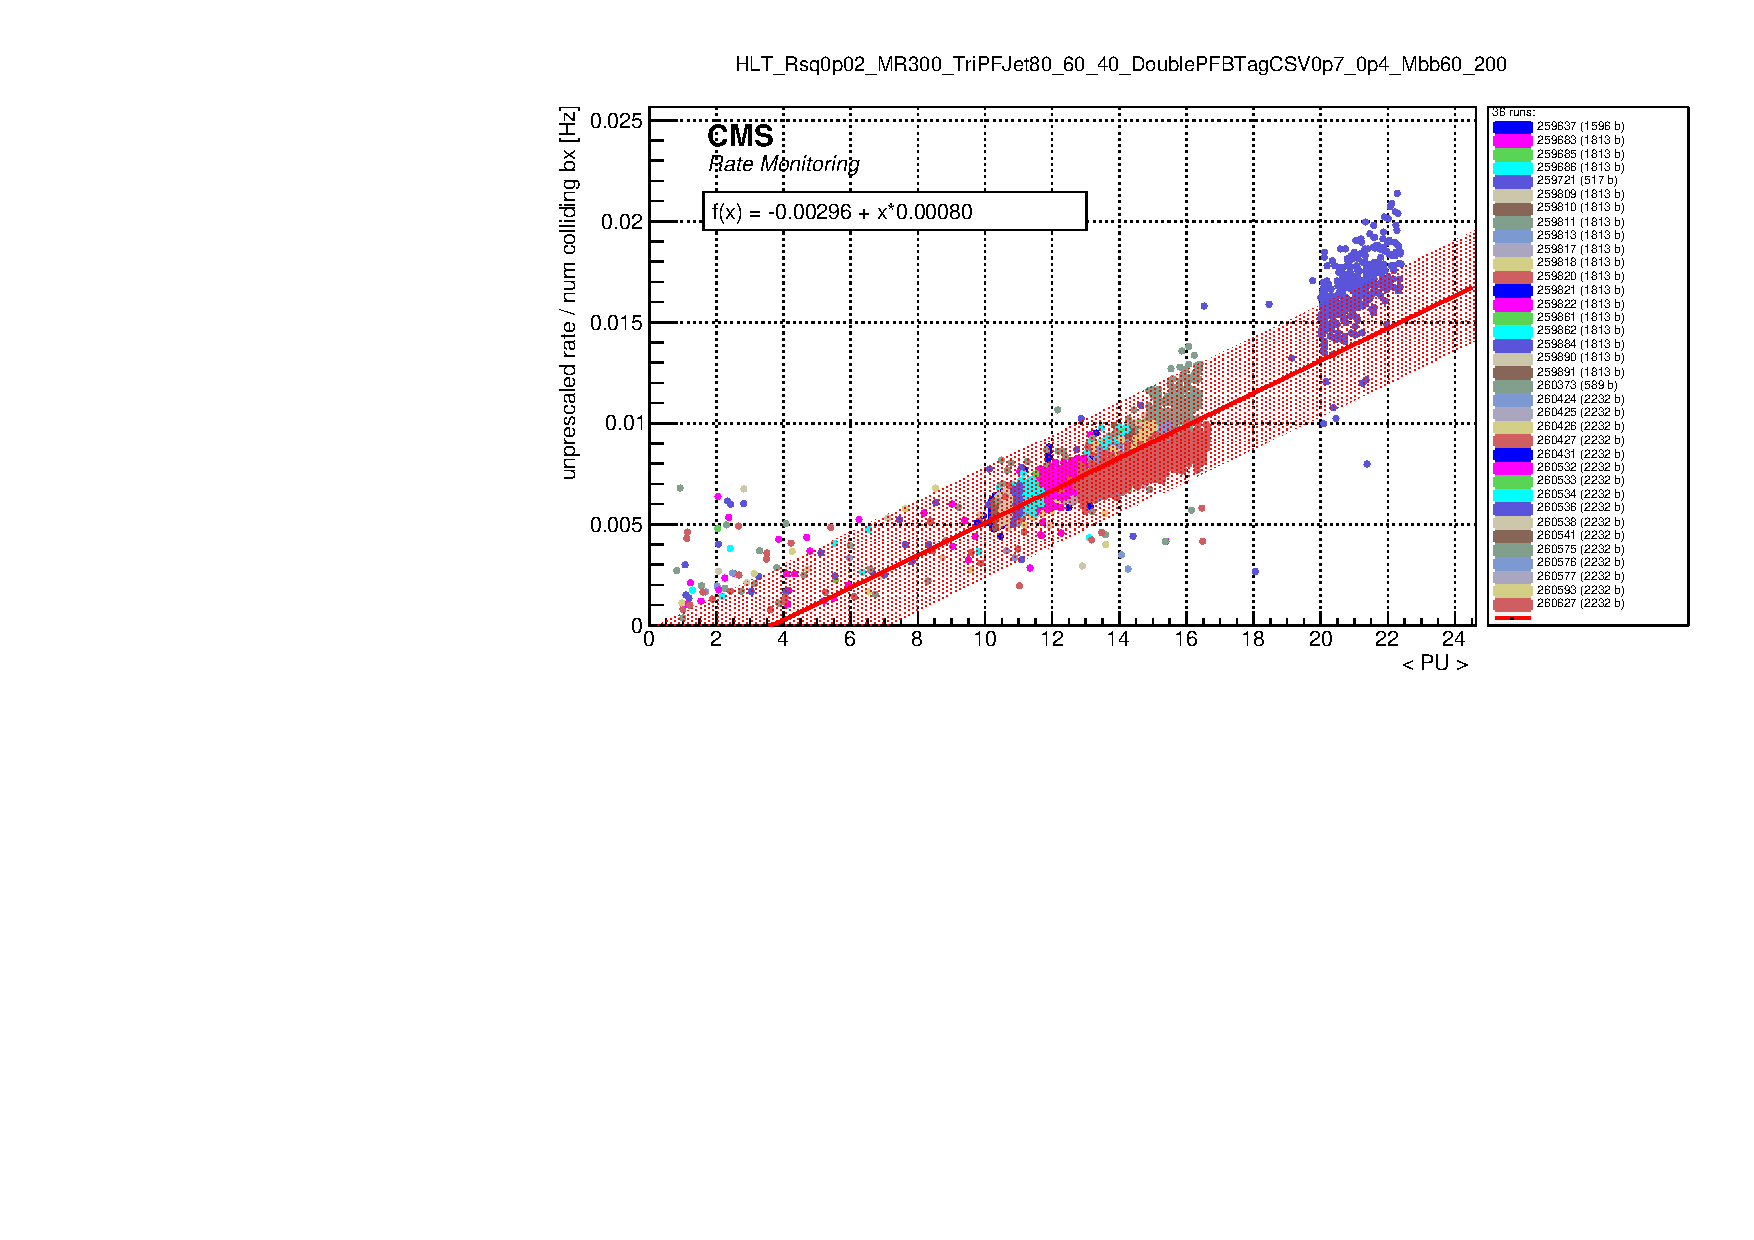
\includegraphics[width=0.49\textwidth]{figs/hlt13TeV/nonlinear/HLT_Rsq0p02_MR300_TriPFJet80_60_40_DoublePFBTagCSV0p7_0p4_Mbb60_200_instLumi_vs_rawRate.pdf}\\
(c) & (d)
\end{tabular}
\caption{\label{fig:HLTpileup} Pileup dependence of the razor triggers.}
\end{figure}


